%\documentclass[11pt,a5paper,landscape]{lerntheke}
\documentclass[12pt,a5paper,landscape]{scrartcl}

\usepackage{vorschule}
\PassOptionsToPackage{dvipsnames}{xcolor}
\usepackage[
    typ=ohne,
    fach=Mathematik,
    lerngruppe={6},
    nummer=1,
    module={Symbole,Lizenzen},
    seitenzahlen=keine,
    farbig,
    lizenz=cc-by-nc-sa-4,
]{schule}

\usepackage[
	typ=lerntheke,
	kuerzel=Ngb,
	reihe={Bruchrechnung},
	version={0.1 (2019-11-07)},
]{ngbschule}

\author{J. Neugebauer}
\title{Bruchrechnung}
\date{\Heute}

\makeatletter
\NewDocumentCommand \tikzRechteck {O{} D(){0,0} m} {\draw[#1] (#2) |- +(#3) |- (#2);}
\NewDocumentCommand \tikzQuadrat {O{} D(){0,0} m} {\draw[#1] (#2) |- +(#3,#3) |- (#2);}

\def\tikzAnteilFarbe{black!20}

\newcounter{ngb@anteile}
\NewDocumentCommand \tikzAnteile {s >{\SplitArgument{1}{,}}D(){0,0} >{\SplitArgument{1}{,}}o m m m} {%
	\IfNoValueTF{#3}{%
		\IfBooleanTF{#1}{%
			\@tikzAnteileZeichnen #2 {#4} {#5} {#4} {#5} {#6-(#4*#5)+1}
		}{%
			\@tikzAnteileZeichnen #2 {#4} {#5} {#4} {#5} {#6}
		}
	}{%
		\IfBooleanTF{#1}{%
			\@tikzAnteileZeichnen #2 #3 {#4} {#5} {#6-(#4*#5)+1}
		}{%
			\@tikzAnteileZeichnen #2 #3 {#4} {#5} {#6}
		}
	}
}
\NewDocumentCommand \@tikzAnteileZeichnen {m m m m m m m}{%
	\pgfmathsetmacro \xMax {#5-1}
	\pgfmathsetmacro \yMax {#6-1}
	\pgfmathsetmacro \xs {#3/#5}
	\pgfmathsetmacro \ys {#4/#6}
	\pgfmathsetmacro \d {sign(#7)*-1}
	\setcounter{ngb@anteile}{#7-1}
	\tikzRechteck(#1,#2){#3,#4};
	\foreach \x in {0,...,\xMax} {%
		\foreach \y in {0,...,\yMax} {%
			\ifnum\value{ngb@anteile}<0
				\tikzRechteck(#1+\x*\xs,#2+\y*\ys){\xs,\ys};
			\else
				\tikzRechteck[fill=\tikzAnteilFarbe](#1+\x*\xs,#2+\y*\ys){\xs,\ys}
			\fi
			\addtocounter{ngb@anteile}{\d}
		}
	}
}

\NewDocumentCommand \tikzAnteileKreis {s D(){0,0} O{1} m m O{0}} {%
	\pgfmathsetmacro \a {#4}
	\pgfmathsetmacro \b {#5}
	\pgfmathsetmacro \ang {360/#5}
	\pgfmathsetmacro \r {#6}
	\draw (#2) circle (#3);
	\foreach \i in {1,...,\a} {%
		\draw[fill=\tikzAnteilFarbe] (#2) -- +({\i*\ang+\r}:#3) arc ({\i*\ang+\r}:{(\i+1)*\ang+\r}:#3) -- cycle;
	}
	\foreach \i in {\a,...,\b} {%
		\draw (#2) -- +({\i*\ang+\r}:#3);
	}
}
\makeatother

\def\clrLsg{\color{orange}}
\def\tclrLsg#1{\textcolor{orange}{#1}}

%\usepackage{pgfmorepages}
%\pgfmorepagesloadextralayouts
%\pgfpagesuselayout{4 on 2, odd then even}[a4paper]

\begin{document}
	\begin{hilfekarte}{Bruchzahlen}{bruchzahlen}
		Brüche beschreiben Anteile von einem Ganzen.
		
		Zum Beispiel \enquote{3 von 4} $= \frac{3}{4} =$ \begin{tikzpicture}[baseline=-3pt,scale=.5]\tikzAnteileKreis{3}{4}\end{tikzpicture}
		
		\begin{tikzpicture}
				
		\end{tikzpicture}
		
		Wir Teilen \emph{das Ganze} in so viele \emph{gleichgroße Teile}, wie im \textbf{Nenner} steht und nehmen von diesen Teilen so viele, wie im \textbf{Zähler} steht.
		
		\vspace{1cm}
		Anteile können auf verschiedene Arten dargestellt werden:
		\begin{multicols}{2}
			Als Bruchzahl: $\frac{3}{4}$
			
			\bigskip
			Als Division: $3:4$
			
			Als Prozentzahl: $\prozent{75}$
			
			\bigskip
			Als \enquote{von} Satz: \enquote{3 von 4}
		\end{multicols}
	\end{hilfekarte}
		
	\begin{hilfekarte}{Kürzen und erweitern}{kuerzen}
		Haben der \textbf{Nenner} und der \textbf{Zähler} eines Bruchs einen gemeinsamen
		\emph{Teiler}, dann kann der Bruch \emph{gekürzt} werden. Der Anteil bleibt dabei gleich.
		
		\vspace{1cm}
		Beim Kürzen wird der \textbf{Zähler} und der \textbf{Nenner} durch denselben \emph{Teiler} dividiert.
		
		\begin{multicols}{2}
			\[ \frac{12}{42} = \frac{2\cdot 6}{7\cdot 6} = \frac{2}{7} \]
			
			\begin{center}
				\begin{tikzpicture}[scale=.5,baseline=3mm]
				\tikzAnteile[5,2]{7}{6}{12}
				\end{tikzpicture} = \begin{tikzpicture}[scale=.5,baseline=3mm]
				\tikzAnteile[5,2]{7}{1}{2}
				\end{tikzpicture}
			\end{center}
		\end{multicols}
		
		\vspace{1cm}
		Umgekehrt kann ein Bruch beliebig \emph{erweitert} werden, indem der \textbf{Zähler} und der \textbf{Nenner} mit demselben Faktor multipliziert werden.
		
		\begin{multicols}{2}
			\[ \frac{3}{8} = \frac{3\cdot 4}{8\cdot 4} = \frac{12}{32} \]
			
			\begin{center}
				\begin{tikzpicture}[scale=.5,baseline=3mm]
				\tikzAnteile[5,2]{4}{2}{3}
				\end{tikzpicture} = \begin{tikzpicture}[scale=.5,baseline=3mm]
				\tikzAnteile[5,2]{4}{8}{12}
				\end{tikzpicture}
			\end{center}
		\end{multicols}
	\end{hilfekarte}
		
	\begin{hilfekarte}{Brüche addieren und subtrahieren}{addition}
		Brüche addieren ist ganz einfach, wenn sie denselben \emph{Nenner} haben.
		\begin{multicols}{2}
			\[ \frac{1}{6} + \frac{4}{6} = \frac{5}{6} \]
			
			\begin{center}
				\begin{tikzpicture}[scale=.5,baseline=3mm]
				\tikzAnteile*{3}{2}{1}
				\end{tikzpicture} + \begin{tikzpicture}[scale=.5,baseline=3mm]
				\tikzAnteile{3}{2}{4}
				\end{tikzpicture} = \begin{tikzpicture}[scale=.5,baseline=3mm]
				\tikzAnteile{3}{2}{5}
				\end{tikzpicture}
			\end{center}
		\end{multicols}
		\vspace{1cm}
		
		Sind die \emph{Nenner} verschieden, dann kannst du sie durch \emph{kürzen} und \emph{erweitern} auf denselben \emph{Nenner} bringen.
		
		\[ \frac{6}{12} + \frac{3}{8} = \frac{12}{24} + \frac{9}{24} = \frac{21}{24} \]
		
		\begin{center}
			 \tikz[scale=.5,baseline=6mm]{\tikzAnteile[4,3]{4}{3}{6}} +
			\tikz[scale=.5,baseline=6mm]{\tikzAnteile[4,3]{2}{4}{3}} = 
			\tikz[scale=.5,baseline=6mm]{\tikzAnteile[4,3]{6}{4}{12}} + 
			\tikz[scale=.5,baseline=6mm]{\tikzAnteile[4,3]{6}{4}{0}\tikzAnteile[2,2.25]{3}{3}{9}} = 
			\tikz[scale=.5,baseline=6mm]{\tikzAnteile[4,3]{6}{4}{12}\tikzAnteile(2,0)[2,2.25]{3}{3}{9}}
		\end{center}
		
		Die Subtraktion geht genauso.
	\end{hilfekarte}

	\begin{hilfekarte}{Brüche gleichnamig machen}{gleichnamig}
		Du kannst Brüche immer \textbf{gleichnamig} machen, indem du jeden Bruch mit dem \emph{Nenner} des anderen Bruchs \emph{erweiterst}:
		
		\[ \frac{2}{3} + \frac{4}{5} = \frac{2\cdot 5}{3\cdot 5} + \frac{4\cdot 3}{5\cdot 3} = \frac{10}{15} + \frac{12}{15} = \frac{22}{15} \]
		
		\vspace{2cm}
		Manchmal gibt es aber auch einen kleineren Nenner, auf den du beide Brüche bringen kannst. Der kleinste gemeinsame Nenner heißt \emph{Hauptnenner}.
		
		\[ \frac{3}{5} + \frac{12}{45} = \frac{3\cdot 3}{5\cdot 3} + \frac{12 : 3}{45 : 3} = \frac{9}{15} + \frac{4}{15} = \frac{13}{15} \]
	\end{hilfekarte}
	
	\begin{hilfekarte}{Multiplikation von Brüchen}{multiplikation}
		Die \emph{Multiplikation} von Brüchen ist ganz einfach:
		
		\begin{center}\itshape
			Zähler mal Zähler und Nenner mal Nenner
		\end{center}
		\[ \frac{2}{3}\cdot \frac{4}{5} = \frac{2\cdot 4}{3\cdot 5} = \frac{8}{15} \]
		
		\vspace{1cm}
		Ein Anteil wie \enquote{$\tfrac{1}{4}$ von 20} ist eigentlich eine Multiplikationsaufgabe:
		\[ \frac{1}{4}\cdot 20 = \frac{1}{4}\cdot \frac{20}{1} = \frac{20}{4} = 5 \]
	\end{hilfekarte}
	
	\begin{hilfekarte}{Division von Brüchen}{division}
		Die \emph{Division} von Brüchen ist mit einem Trick ganz einfach:
		
		\begin{center}
			Du dividierst durch einen Bruch, indem du mit dem \emph{Kehrwert} des Bruchs multiplizierst.
		\end{center}
		\[ \frac{2}{3}: \frac{5}{4} \overset{\text{Kehrwert}}{\underset{\text{Aus }:
		\text{ wird }\cdot}{=}} \frac{2}{3}\cdot  \frac{4}{5} = \frac{2\cdot 4}{3\cdot 5} = \frac{8}{15} \]
		
		\vspace{1cm}
		Jetzt musst du nur noch wissen, was der \emph{Kehrwert} ist:
		\begin{center}
			Beim \emph{Kehrwert} vertauscht du Zähler und Nenner.
		\end{center}
		\[ \frac{2}{9} \rightarrow \frac{9}{2} \qquad \frac{4}{5} \rightarrow \frac{5}{4}\]
	\end{hilfekarte}
		
	\begin{karte1}{Arten von Brüchen}\hilfeMarke{bruchzahlen}
		\setlength{\columnseprule}{.5pt}\small
		\begin{multicols}{2}
		Es gibt verschiedene Arten von Brüchen:
		\begin{smalldescription}
			\item[Echte Brüche] Bei echten Brüchen ist der \emph{Zähler} kleiner als der \emph{Nenner}. ($\tfrac{2}{3}$)
			\item[Stammbrüche] Brüche mit dem Zähler $1$ heißen Stammbrüche.
 ($\tfrac{1}{7}$)
 			\item[Unechte Brüche] Bei unechten Brüchen ist der \emph{Zähler} größer oder gleich dem \emph{Nenner}. Unechte Brüche sind größer als ein Ganzes. ($\tfrac{23}{4}$)
			\item[Gemischte Brüche] Unechte Brüche lassen sich auch als gemischte Brüche schreiben. Dazu wird der Zähler mit Rest durch den Nenner geteilt. Das Ergebnis wird vor den Bruch geschrieben, der Rest wird der neue Zähler. ($\tfrac{14}{6} = 2\tfrac{2}{6}$)
		\end{smalldescription}
		
		\columnbreak
		\textbf{Aufgabe}\\
		Notiere in deinem Heft eine Tabelle und ordne die Brüche passend zu. Überlege dir zu jeder Bruchart auch drei eigene Beispiele.
		
		\begin{center}\footnotesize
			\begin{tabular}{c|c}\hline
				Echte Brüche & \hspace{2cm} \\\hline
				Stammbrüche & \\\hline
				Unechte Brüche & \\\hline
				Gemischte Brüche & \\\hline
			\end{tabular}
	
			\normalsize
			\begin{tikzpicture}
				\node at (0,0) {$\frac{1}{6}$};
				\node at (1,2) {$\frac{14}{12}$};
				\node at (-1,2.5) {$\frac{3}{5}$};
				\node at (-1.5,-1) {$5\frac{1}{4}$};
				\node at (3.5,0) {$2\frac{2}{7}$};
				\node at (3,-1) {$\frac{19}{52}$};
				\node at (3,1.5) {$\frac{43}{19}$};
				\node at (2,-.5) {$\frac{1}{10}$};
				\node at (2,1.2) {$1\frac{1}{12}$};
			\end{tikzpicture}
		\end{center}
		\end{multicols}
	\end{karte1}
	
	\begin{loesungskarte}
		\begin{center}
			\begin{tabular}{|c|c|}\hline
				Echte Brüche & $\tfrac{3}{5}\quad \tfrac{19}{52}$ \\\hline
				Stammbrüche & $\tfrac{1}{6}\quad \tfrac{1}{10}$ \\\hline
				Unechte Brüche & $\tfrac{14}{12}\quad \tfrac{43}{19}$ \\\hline
				Gemischte Brüche & $5\tfrac{1}{4}\quad 2\tfrac{2}{7}\quad 1\tfrac{1}{12}$ \\\hline
			\end{tabular}
		\end{center}
	\end{loesungskarte}
	
	\begin{karte1}{Prozentzahlen}
		\hilfeMarke{kuerzen}
		Einen Hundertstelbruch kannst du auch als \textbf{Prozentzahl} schreiben. Gegebenenfalls musst du den Bruch zuerst durch kürzen und erweitern auf den \emph{Nenner} \num{100} bringen.
		
		\[ \frac{7}{20} = \frac{35}{100} = \prozent{35} \]
		
		\begin{enumerate}
			\item Schreibe als Prozentzahl.
			\begin{tasks}(4)
				\task $\dfrac{15}{100}$
				\task $\dfrac{3}{20}$
				\task $\dfrac{1}{5}$
				\task $\dfrac{9}{10}$
				\task $\dfrac{200}{500}$
				\task $\dfrac{40}{25}$
				\task $\dfrac{30}{30}$
				\task $\dfrac{20}{80}$
			\end{tasks}
			
			\item Schreibe als vollständig gekürzten Bruch.
			\begin{tasks}(4)
				\task $\prozent{75}$
				\task $\prozent{30}$
				\task $\prozent{14}$
				\task $\prozent{85}$
			\end{tasks}
		\end{enumerate}
	\end{karte1}
	
	\begin{loesungskarte}
		\vspace*{1cm}
		\begin{enumerate}
			\item\begin{tasks}(4)
				\task $\dfrac{15}{100} = \clrLsg\prozent{15}$
				\task $\dfrac{3}{20} = \clrLsg\prozent{15}$
				\task $\dfrac{1}{5} = \clrLsg\prozent{20}$
				\task $\dfrac{9}{10} = \clrLsg\prozent{90}$
				\task $\dfrac{200}{500} = \clrLsg\prozent{40}$
				\task $\dfrac{40}{25} = \clrLsg\prozent{160}$
				\task $\dfrac{30}{30} = \clrLsg\prozent{100}$
				\task $\dfrac{20}{80} = \clrLsg\prozent{25}$
			\end{tasks}
			
			\vspace{1cm}
			\item\begin{tasks}(4)
				\task $\prozent{75} = \clrLsg\dfrac{3}{4}$
				\task $\prozent{30} = \clrLsg\dfrac{3}{10}$
				\task $\prozent{14} = \clrLsg\dfrac{7}{50}$
				\task $\prozent{85} = \clrLsg\dfrac{17}{20}$
			\end{tasks}
		\end{enumerate}
	\end{loesungskarte}
	
	\begin{karte1}{Anteile berechnen}\hilfeMarke{multiplizieren}
		Berechne im Kopf.
		
		\begin{tasks}(4)
			\task $\dfrac{2}{3}$ von \SI{21}{\gram}
			\task $\dfrac{3}{5}$ von \SI{65}{\gram}
			\task $\dfrac{13}{15}$ von \SI{90}{\milli\liter}
			\task $\dfrac{3}{4}$ von \SI{36}{\meter}
			\task $\dfrac{5}{6}$ von \SI{180}{\kilo\gram}
			\task $\dfrac{15}{20}$ von \SI{300}{\hectare}
			\task $\dfrac{3}{7}$ von \SI{42}{\meter}
			\task $\dfrac{3}{9}$ von \SI{36}{\liter}
			\task $\dfrac{13}{25}$ von \EUR{500}
			\task $\dfrac{4}{5}$ von \SI{35}{\kilo\gram}
			\task $\dfrac{5}{12}$ von \SI{48}{\minute}
			\task $\dfrac{6}{125}$ von \SI{375}{\hour}
		\end{tasks}
	\end{karte1}
	
	\begin{loesungskarte}
		\vspace*{1cm}
		\begin{tasks}(4)
			\task \SI{14}{\gram}
			\task \SI{39}{\gram}
			\task \SI{78}{\milli\liter}
			\task \SI{27}{\meter}
			\task \SI{150}{\kilo\gram}
			\task \SI{225}{\hectare}
			\task \SI{18}{\meter}
			\task \SI{12}{\liter}
			\task \EUR{260}
			\task \SI{28}{\kilo\gram}
			\task \SI{20}{\minute}
			\task \SI{18}{\hour}
		\end{tasks}
	\end{loesungskarte}
	
	\begin{karte2}{Das Ganze berechnen}\hilfeMarke{multiplikation}\hilfeMarke{division}
		Berechne das Ganze, wenn nur ein Bruchteil angegeben ist.
		
		\begin{tasks}(4)
			\task $\dfrac{1}{4}$ sind \SI{50}{\kilo\gram}
			\task $\dfrac{2}{4}$ sind \SI{30}{Stück}
			\task $\dfrac{3}{4}$ sind \SI{150}{\square\meter}
			\task $\dfrac{1}{3}$ sind \SI{150}{\kilo\meter}
			\task $\dfrac{1}{8}$ sind \SI{20}{\kilo\gram}
			\task $\dfrac{1}{7}$ sind \SI{4}{\hecto\liter}
			\task $\dfrac{3}{8}$ sind \SI{27}{\hour}
			\task $\dfrac{2}{9}$ sind \EUR{14}
			\task $\dfrac{5}{11}$ sind \SI{45}{\kilo\gram}
			\task $\dfrac{11}{15}$ sind \SI{44}{\kilo\meter}
			\task $\dfrac{5}{6}$ sind \SI{15}{\hour}
			\task $\dfrac{2}{3}$ sind \SI{18}{\kilo\meter}
		\end{tasks}
	\end{karte2}
	
	\begin{loesungskarte}
		\begin{tasks}(4)
			\task \SI{200}{\kilo\gram}
			\task \SI{60}{Stück}
			\task \SI{200}{\square\meter}
			\task \SI{450}{\kilo\meter}
			\task \SI{160}{\kilo\gram}
			\task \SI{28}{\hecto\liter}
			\task \SI{72}{\hour}
			\task \EUR{63}
			\task \SI{99}{\kilo\gram}
			\task \SI{60}{\kilo\meter}
			\task \SI{18}{\hour}
			\task \SI{27}{\kilo\meter}
		\end{tasks}
	\end{loesungskarte}
	
	\begin{karte1}{Brüche addieren und subtrahieren}\hilfeMarke{addition}
		Rechne schriftlich im Heft.
		\begin{tasks}(4)
			\task $\dfrac{7}{8} + \dfrac{3}{5} + \dfrac{2}{1}$
			\task $\dfrac{1}{2} - \dfrac{1}{4} + \dfrac{7}{10}$
			\task $\dfrac{5}{14} - \dfrac{1}{7} + \dfrac{3}{2}$
			\task $\dfrac{7}{8} - \dfrac{3}{4} + \dfrac{5}{12}$
			\task $\dfrac{1}{1} + \dfrac{1}{2} + \dfrac{1}{3} \dfrac{1}{4}$
			\task $\dfrac{1}{2} + \dfrac{1}{4} + \dfrac{1}{8} + \dfrac{1}{16}$
		\end{tasks}
	\end{karte1}
	
	\begin{loesungskarte}
		\vspace*{1cm}
		\begin{tasks}(4)
			\task $3\dfrac{19}{40}$
			\task $\dfrac{19}{20}$
			\task $1\dfrac{5}{7}$
			\task $\dfrac{13}{24}$
			\task $2\dfrac{1}{12}$
			\task $\dfrac{15}{16}$
		\end{tasks}
	\end{loesungskarte}
	
	\begin{karte1}{Bruchterme I}\hilfeMarke{addition}
		Welche Zahl muss man für $x$ einsetzen, damit die Rechnung stimmt?
	
		\vspace{1cm}
		\begin{tasks}(3)
			\task $\dfrac{3}{8} + \dfrac{x}{8} = \dfrac{5}{8}$
			\task $\dfrac{9}{13} - \dfrac{x}{13} = \dfrac{3}{13}$
			\task $\dfrac{x}{29} + \dfrac{7}{29} = \dfrac{15}{29}$
			\task $\dfrac{x}{7} - \dfrac{6}{7} = \dfrac{4}{7}$
			\task $\dfrac{3}{4} + \dfrac{x}{2} = \dfrac{5}{4}$
			\task $\dfrac{2}{3} - \dfrac{x}{6} = \dfrac{1}{6}$
			\task $\dfrac{1}{5} + \dfrac{1}{x} = \dfrac{3}{10}$
			\task $\dfrac{8}{9} - \dfrac{x}{27} = \dfrac{5}{9}$
			\task $\dfrac{x}{2} + \dfrac{12}{26} = \dfrac{25}{26}$
		\end{tasks}
		
		\infotext{$2,6,8,10,1,3,10,9,1$}
	\end{karte1}
		
	% Leere Rückseite
	\leereKarte
	
	\begin{karte2}{Bruchterme II}\hilfeMarke{multiplikation}\hilfeMarke{division}
		Welche Zahl muss man für $x$ einsetzen, damit die Rechnung stimmt?
	
		\vspace{1cm}
		\begin{tasks}(3)
			\task $\dfrac{1}{2} : x = \dfrac{1}{4}$
			\task $\dfrac{1}{2}\cdot x = 2$
			\task $\dfrac{3}{5} : x = \dfrac{1}{5}$
			\task $\dfrac{3}{5}\cdot x = 3$
			\task $\dfrac{x}{3} : \dfrac{5}{3} = \dfrac{1}{5}$
			\task $\dfrac{x}{4}\cdot \dfrac{2}{5} = \frac{3}{10}$
			\task $\dfrac{1}{11} : \dfrac{x}{11} = \dfrac{1}{3}$
			\task $\dfrac{2}{7}\cdot \dfrac{x}{4} = \dfrac{3}{14}$
		\end{tasks}
		
		\infotext{$2,4,3,5,1,3,3,3$}
	\end{karte2}
			
	% Leere Rückseite
	\leereKarte
	
	\begin{karte2}{Rechenmauer (Addition)}
		\begin{enumeratea}
			\item\centering\begin{tikzpicture}[baseline=(current bounding box.north)]
				\draw (0,0) |- (6,1) |- (0,0);
				\draw (1,1) |- (5,2) |- (1,1);
				\draw (2,2) |- (4,3) |- (2,2);
				\draw (-1,0) |- (7,-1) |- (-1,0);
				\draw (2,0) -- +(0,1);
				\draw (4,0) -- +(0,1);
				\draw (3,1) -- +(0,1);
				\draw (1,0) -- +(0,-1);
				\draw (3,0) -- +(0,-1);
				\draw (5,0) -- +(0,-1);
				
				\node (a) at (0,-.5) {\Large$\tfrac{1}{8}$};
				\node (b) at (2,-.5) {\Large$\tfrac{3}{8}$};
				\node (d) at (4,1.5) {\Large$\tfrac{20}{8}$};
				\node (d) at (3,2.5) {\Large$\tfrac{32}{8}$};
			\end{tikzpicture}
			
			\item\centering\begin{tikzpicture}[baseline=(current bounding box.north)]
				\draw (0,0) |- (6,1) |- (0,0);
				\draw (1,1) |- (5,2) |- (1,1);
				\draw (2,2) |- (4,3) |- (2,2);
				\draw (-1,0) |- (7,-1) |- (-1,0);
				\draw (2,0) -- +(0,1);
				\draw (4,0) -- +(0,1);
				\draw (3,1) -- +(0,1);
				\draw (1,0) -- +(0,-1);
				\draw (3,0) -- +(0,-1);
				\draw (5,0) -- +(0,-1);
				
				\node (a) at (0,-.5) {\Large$\tfrac{2}{10}$};
				\node (a) at (4,-.5) {\Large$\tfrac{3}{10}$};
				\node (a) at (6,-.5) {\Large$\tfrac{5}{10}$};
				\node (a) at (3,.5) {\Large$\tfrac{7}{10}$};
			\end{tikzpicture}
		\end{enumeratea}
	\end{karte2}
	
	\begin{loesungskarte}
		\begin{enumeratea}
			\item\centering\begin{tikzpicture}
				\draw (0,0) |- (6,1) |- (0,0);
				\draw (1,1) |- (5,2) |- (1,1);
				\draw (2,2) |- (4,3) |- (2,2);
				\draw (-1,0) |- (7,-1) |- (-1,0);
				\draw (2,0) -- +(0,1);
				\draw (4,0) -- +(0,1);
				\draw (3,1) -- +(0,1);
				\draw (1,0) -- +(0,-1);
				\draw (3,0) -- +(0,-1);
				\draw (5,0) -- +(0,-1);
				
				\node (a) at (0,-.5) {\Large$\tfrac{1}{8}$};
				\node (b) at (2,-.5) {\Large$\tfrac{3}{8}$};
				\node (d) at (4,1.5) {\Large$\tfrac{20}{8}$};
				\node (d) at (3,2.5) {\Large$\tfrac{32}{8}$};
				
				\node (a) at (4,-.5) {\Large\clrLsg$\tfrac{5}{8}$};
				\node (a) at (6,-.5) {\Large\clrLsg$\tfrac{7}{8}$};
				\node (a) at (1,.5) {\Large\clrLsg$\tfrac{4}{8}$};
				\node (a) at (3,.5) {\Large\clrLsg$\tfrac{8}{8}$};
				\node (a) at (5,.5) {\Large\clrLsg$\tfrac{12}{8}$};
				\node (a) at (2,1.5) {\Large\clrLsg$\tfrac{12}{8}$};
			\end{tikzpicture}
			
			\item\centering\begin{tikzpicture}
				\draw (0,0) |- (6,1) |- (0,0);
				\draw (1,1) |- (5,2) |- (1,1);
				\draw (2,2) |- (4,3) |- (2,2);
				\draw (-1,0) |- (7,-1) |- (-1,0);
				\draw (2,0) -- +(0,1);
				\draw (4,0) -- +(0,1);
				\draw (3,1) -- +(0,1);
				\draw (1,0) -- +(0,-1);
				\draw (3,0) -- +(0,-1);
				\draw (5,0) -- +(0,-1);
				
				\node (a) at (0,-.5) {\Large$\tfrac{2}{10}$};
				\node (a) at (4,-.5) {\Large$\tfrac{3}{10}$};
				\node (a) at (6,-.5) {\Large$\tfrac{5}{10}$};
				\node (a) at (3,.5) {\Large$\tfrac{7}{10}$};

				\node (a) at (2,-.5) {\Large\clrLsg$\tfrac{4}{10}$};
				\node (a) at (1,.5) {\Large\clrLsg$\tfrac{6}{10}$};
				\node (a) at (5,.5) {\Large\clrLsg$\tfrac{8}{10}$};
				\node (a) at (2,1.5) {\Large\clrLsg$\tfrac{13}{10}$};
				\node (a) at (4,1.5) {\Large\clrLsg$\tfrac{15}{10}$};
				\node (a) at (3,2.5) {\Large\clrLsg$\tfrac{28}{10}$};
			\end{tikzpicture}
		\end{enumeratea}
	\end{loesungskarte}
	
	\begin{karte1}{Bruchteile berechnen I}\hilfeMarke{multiplikation}
%		Berechne im Kopf.
%		
%		\vspace{1cm}
%		\begin{tasks}(4)
%			\task $\dfrac{2}{3}$ von \SI{21}{\gram}
%			\task $\dfrac{3}{4}$ von \SI{36}{\meter}
%			\task $\dfrac{3}{7}$ von \SI{42}{\meter}
%			\task $\dfrac{4}{5}$ von \SI{35}{\kilo\gram}
%			\task $\dfrac{3}{5}$ von \SI{65}{\gram}
%			\task $\dfrac{5}{6}$ von \SI{180}{\kilo\gram}
%			\task $\dfrac{3}{9}$ von \SI{36}{\liter}
%			\task $\dfrac{5}{12}$ von \SI{48}{\minute}
%			\task $\dfrac{13}{15}$ von \SI{90}{\milli\meter}
%			\task $\dfrac{15}{20}$ von \SI{300}{\hectare}
%			\task $\dfrac{13}{25}$ von \EUR{500}
%			\task $\dfrac{6}{125}$ von \SI{375}{\hour}
%		\end{tasks}
	\end{karte1}
	
	\leereKarte
%	\begin{loesungskarte}
%		\begin{tasks}(4)
%			\task $\dfrac{2}{3}$ von \SI{21}{\gram} = \clrLsg\SI{14}{\gram}
%			\task $\dfrac{3}{4}$ von \SI{36}{\meter} = \clrLsg\SI{27}{\meter}
%			\task $\dfrac{3}{7}$ von \SI{42}{\meter} = \clrLsg\SI{18}{\meter}
%			\task $\dfrac{4}{5}$ von \SI{35}{\kilo\gram} = \clrLsg\SI{28}{\kilo\gram}
%			\task $\dfrac{3}{5}$ von \SI{65}{\gram} = \clrLsg\SI{39}{\gram}
%			\task $\dfrac{5}{6}$ von \SI{180}{\kilo\gram} = \clrLsg\SI{150}{\kilo\gram}
%			\task $\dfrac{3}{9}$ von \SI{36}{\liter} = \clrLsg\SI{12}{\liter}
%			\task $\dfrac{5}{12}$ von \SI{48}{\minute} = \clrLsg\SI{20}{\minute}
%			\task $\dfrac{13}{15}$ von \SI{90}{\milli\meter} = \clrLsg\SI{68}{\milli\liter}
%			\task $\dfrac{15}{20}$ von \SI{300}{\hectare} = \clrLsg\SI{225}{\hectare}
%			\task $\dfrac{13}{25}$ von \EUR{500} = \clrLsg\EUR{260}
%			\task $\dfrac{6}{125}$ von \SI{375}{\hour} = \clrLsg\SI{18}{\hour}
%		\end{tasks}
%	\end{loesungskarte}
	
	\begin{karte2}{Anteile berechnen II}
		\begin{enumerate}
			\item Wie hoch ragt ein \SI{28}{\centi\meter} dickes Eisstück aus dem Wasser, wenn nur $\dfrac{1}{7}$ des Eises zu sehen ist?
			
			\item Für ein Klassenfest hatte die 6c folgendes eingekauft:
			\begin{itemize}
				\item 63 Würstchen
				\item 90 Flaschen Cola
				\item 24 Tüten Chips
			\end{itemize}
			\begin{enumeratea}
				\item Am Ende sind $\dfrac{1}{9}$ der Würstchen und $\dfrac{5}{18}$ der Cola übrig. Berechne den Anteil. 
				\item Von den Chips bleiben \num{4} Tüten übrig. Welcher Bruchteil war das?
			\end{enumeratea}
			
			\item Ca. $\dfrac{4}{5}$ eines Apfels sind Wasser, $\dfrac{1}{12}$ des Gewichts sind Fruchtzucker. Wie viele Gramm Wasser und Zucker enthält ein Apfel von \SI{120}{\gram} (\SI{180}{\gram},  \SI{240}{\gram})?
		\end{enumerate}
	\end{karte2}
	
	\begin{loesungskarte}
		\begin{enumerate}
			\item \SI{4}{\centi\meter}
			
			\item 7 Würstchen, 25 Flaschen Cola und $\dfrac{1}{6}$ der Tüten Chips
			
			\item \begin{itemize}
				\item \SI{120}{\gram}-Apfel:\hspace{1cm} \SI{96}{\gram} Wasser, \SI{10}{\gram} Fruchtzucker
				\item \SI{180}{\gram}-Apfel:\hspace{1cm} \SI{144}{\gram} Wasser, \SI{50}{\gram} Fruchtzucker
				\item \SI{240}{\gram}-Apfel:\hspace{1cm} \SI{192}{\gram} Wasser, \SI{20}{\gram} Fruchtzucker
			\end{itemize}
		\end{enumerate}
	\end{loesungskarte}
	
	\begin{karte3}{Punktrechnung bei Brüchen}\hilfeMarke{multiplikation}\hilfeMarke{division}
		Rechne schriftlich im Heft.
		\begin{enumerate}
			\item \begin{tasks}(4)
				\task $9\dfrac{3}{8}\cdot \dfrac{4}{25}$
				\task $1\dfrac{5}{16}\cdot \dfrac{3}{3}$
				\task $7\dfrac{1}{3}\cdot \dfrac{1}{2}$
				\task $5\dfrac{2}{5}\cdot \dfrac{7}{9}$
				\task $\dfrac{9}{10}\cdot 1\dfrac{3}{4}$
				\task $\dfrac{3}{4}\cdot 5\dfrac{5}{6}$
				\task $\dfrac{4}{5}\cdot 1\dfrac{1}{4}$
				\task $\dfrac{1}{7}\cdot 3\dfrac{1}{2}$
			\end{tasks}
			
			\vspace{2cm}
			\item \begin{tasks}(3)
				\task $4\dfrac{1}{2}\cdot 5\dfrac{2}{3}\cdot 6\dfrac{3}{4}$
				\task $7\dfrac{3}{5}\cdot 10\dfrac{5}{6}\cdot 2\dfrac{1}{2}$
				\task $\dfrac{5}{8}\cdot \dfrac{6}{11}: \dfrac{5}{6}$
				\task $\dfrac{8}{15}\cdot \dfrac{4}{7}: \dfrac{11}{21}$
				\task $11\dfrac{7}{10}: 7\dfrac{4}{5}$
				\task $12\dfrac{3}{5}: 7\dfrac{7}{20}$
			\end{tasks}
		\end{enumerate}
	\end{karte3}
	
	\begin{loesungskarte}
		\begin{enumerate}
			\item \begin{tasks}(4)
				\task \clrLsg$1\frac{1}{2}$
				\task \clrLsg$1\frac{5}{16}$
				\task \clrLsg$3\frac{2}{3}$
				\task \clrLsg$4\frac{1}{5}$
				\task \clrLsg$1\frac{23}{40}$
				\task \clrLsg$4\frac{3}{8}$
				\task \clrLsg$1$
				\task \clrLsg$\frac{1}{2}$
			\end{tasks}
			
			\vspace{2cm}
			\item \begin{tasks}(3)
				\task \clrLsg$4\dfrac{1}{2}\cdot 5\dfrac{2}{3}\cdot 6\dfrac{3}{4}$
				\task \clrLsg$7\dfrac{3}{5}\cdot 10\dfrac{5}{6}\cdot 2\dfrac{1}{2}$
				\task \clrLsg$\dfrac{5}{8}\cdot \dfrac{6}{11}: \dfrac{5}{6})$
				\task \clrLsg$\dfrac{8}{15}\cdot \dfrac{4}{7}: \dfrac{11}{21}$
				\task \clrLsg$11\dfrac{7}{10}: 7\dfrac{4}{5}$
				\task \clrLsg$12\dfrac{3}{5}: 7\dfrac{7}{20}$
			\end{tasks}
		\end{enumerate}
	\end{loesungskarte}
	
	\begin{karte3}[\symPartner]{Brawl Stars}
		\begin{minipage}{.5\textwidth}
			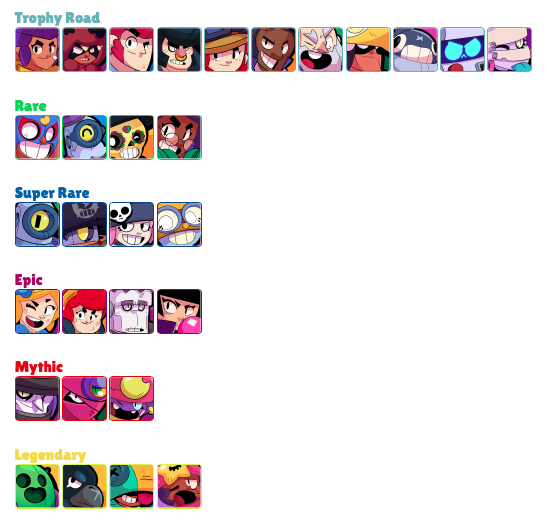
\includegraphics[width=\textwidth]{6.1-LT-Abb_Brawler}
		\end{minipage}\hfill\begin{minipage}{.49\textwidth}
			Links siehst du eine Übersicht aller \emph{Brawler}, die man derzeit in \emph{Brawl Stars} spielen kann.
			
			\begin{smallenumerate}\small
				\item Gebt für jede Brawler-Kategorie an, welcher Anteil aller Brawler ihr angehören.
				
				\item Der Brawler \person{Frank} hat auf Level 1 mit \num{6100} die meisten Lebenspunkte aller Brawler. \person{Tick} hat dagegen nur etwa $\tfrac{9}{25}$ davon (und damit am wenigsten). Wie viel Lebenspunkte hat \person{Tick} ungefähr?
				
				\item Die Brawlerin \person{Piper} kann auf Level 9 maximal \num{1900} Schadenspunkte austeilen. Das sind aber nur \prozent{70} des Schadens den sie erreichen kann, wenn sie ihre Star-Power \emph{Hinterhalt} aktiviert und sich in einem Busch versteckt. Wie hoch ist dann ihr maximaler Schaden ungefähr?
			\end{smallenumerate}
		\end{minipage}
	\end{karte3}
	
	\begin{loesungskarte}
		\begin{multicols}{2}
		\begin{enumeratea}
			\item \begin{smallitemize}
				\item Trophy Road: $\clrLsg\dfrac{11}{30}$
				\item Rare: $\clrLsg\dfrac{4}{30}$
				\item Super Rare: $\clrLsg\dfrac{4}{30}$
				\item Epic: $\clrLsg\dfrac{4}{30}$
				\item Mythic: $\clrLsg\dfrac{3}{30}$
				\item Legendary: $\clrLsg\dfrac{4}{30}$
			\end{smallitemize}
			
			\item Zu berechnen ist, wie viel $\tfrac{9}{25}$ von \num{6100} sind:
			\[ \frac{9}{25}\cdot 6100 = \frac{9\cdot 6100}{25} = \frac{54900}{25} = \clrLsg2196 \]
			
			\item Wenn \num{1900} der Anteil $\prozent{70} = \frac{7}{10}$ vom Ganzen sind, dann kann das Ganze berechnet werden durch:
			\begin{align*}
				1900: \frac{7}{10} &= 1900\cdot \frac{10}{7} = \frac{1900\cdot 10}{7} \\
				&= \frac{19000}{7} = \clrLsg 2714\frac{2}{7}\approx 2714
			\end{align*}
		\end{enumeratea}
		\end{multicols}
	\end{loesungskarte}
	
	\begin{karte3}[\symPartner]{Frozen}
		\begin{wrapfigure}[11]{r}{0pt}
			
\includegraphics[width=3cm]{6.1-LT-Abb_Frozen}
		\end{wrapfigure}
		
		Der Film \emph{Frozen} ist 2013 in die Kinos gekommen und hat große Erfolge gefeiert.
		Bisher hat er weltweit schon weit über \$\num{1200000000} eingespielt (über \num{1,2} Milliarden Dollar).
		
		\begin{enumeratea}\small
			\item Der Produzent Disney war mit den Einnahmen sehr zufrieden, denn die Produktion des Films hatte nur etwa $\tfrac{1}{8}$ davon gekostet. Wie teuer war der Film ungefähr?
			
			\item Alleine am ersten Wochenende nach Veröffentlichung konnte der Film \$\num{400000000} einspielen. Welcher Anteil der gesamten Einnahmen ist das?
			
			\item Im Film soll Prinzessin \person{Elsa} zur Königin gekrönt werden. Bisher musste sie sich ganze \num{13} Jahre im Schloss verstecken. Das waren immerhin \prozent{62} ihres Lebens. Wie alt ist \person{Elsa}, als sie gekrönt werden soll und wie alt war sie, als ihre Familie sich im Schloss eingeschlossen hat? (Rundet das Ergebnis.)
		\end{enumeratea}
		
		\infotext{Image by Mallory Muse from Pixabay }
	\end{karte3}
	
	\begin{loesungskarte}
		\begin{multicols}{2}
		\begin{enumeratea}
			\item Gesucht sind $\dfrac{1}{8}$ von \num{1200000000}.
			\begin{align*}
				\frac{1}{8}\cdot 1200000000 &= \frac{1200000000}{8} \\
					&= 1200000000 : 8 \\
					&= \clrLsg 150000000
			\end{align*}
			
			\item
			\[ \frac{400000000}{1200000000} = \frac{4}{12} = \clrLsg\frac{1}{3} \]
			
			\item Wenn \num{13} Jahre $\prozent{62} = \tfrac{62}{100}$ ihres Lebens sind, dann ist ihr Alter:
			\begin{align*}
				13: \frac{62}{100} &= 13\cdot \frac{100}{62} \\
					&= \frac{13\cdot 100}{62} \\
					&= \frac{1300}{62} = \clrLsg 20\frac{60}{62}\approx 21
			\end{align*}
			Elsa ist also \num{21} Jahre alt. \num{13} Jahre zuvor war sie dann \num{8} Jahre.
		\end{enumeratea}
		\end{multicols}
	\end{loesungskarte}
	
	\begin{karte2}[\symPartner]{Verhältnisse}
		Im Fußball wird in der Tabelle auch das \emph{Torverhältnis} angegeben. Zum Beispiel bedeutet \enquote{6 zu 4}, dass der Verein in den bisher $6$ Tore geschossen und $4$ Tore kassiert hat.
		
		\begin{enumerate}
			\item Wie viele Tore sind in den Spielen des Vereins oben insgesamt gefallen? Welchen Anteil der Tore hat die Mannschaft geschossen? Welchen Anteil hat sie selber rein bekommen?
			\item Schreibe zu den folgenden Torverhältnissen die beiden Brüche auf.
				\begin{tasks}(4)
					\task 8 zu 10
					\task 10 zu 5
					\task 9 zu 3
					\task 3 zu 9
				\end{tasks}
			\item Schreibt jeweils das Torverhältnis auf.
				\begin{tasks}(1)
					\task 4 Tore erhalten und 5 Tore geschossen.
					\task 2 Tore geschossen und 11 Tore erhalten.
					\task Von 14 Toren wurden 5 selber geschossen.
					\task $\dfrac{13}{25}$ der Tore hat die Mannschaft in das eigene Tor bekommen.
				\end{tasks}
		\end{enumerate}
	\end{karte2}
	
	\begin{loesungskarte}
		\begin{enumerate}
			\item Insgesamt sind $6+4=10$ Tore gefallen. $\dfrac{6}{10}$ hat die Mannschaft geschossen und $\dfrac{4}{10}$ haben sie erhalten.
			
			\item\begin{tasks}(4)
				\task $\dfrac{8}{18}, \dfrac{10}{18}$
				\task $\dfrac{10}{15}, \dfrac{5}{15}$
				\task $\dfrac{9}{12}, \dfrac{3}{12}$
				\task $\dfrac{3}{12}, \dfrac{9}{12}$
			\end{tasks}
				
			\item\begin{tasks}(1)
				\task 5 zu 4
				\task 2 zu 11
				\task 5 zu 9
				\task 12 zu 13
			\end{tasks}
		\end{enumerate}
	\end{loesungskarte}

	\begin{karte1}{Brüche ordnen}
		Ordne die Brüche der Größe nach vom Kleinsten zum Größten.
		
		\begin{enumeratea}
			\item \[ \frac{2}{3}\:;\ \frac{1}{2}\:;\ \frac{4}{5}\:;\ \frac{3}{10}\:;\ \frac{5}{6} \]
			
			\item \[ \frac{4}{5}\:;\ \frac{7}{9}\:;\ \frac{14}{15}\:;\ \frac{2}{3}\:;\ \frac{17}{18}\:;\ \frac{13}{20} \]
			
			\item \[ \frac{16}{35}\:;\ \frac{3}{7}\:;\ \frac{4}{5}\:;\ \frac{6}{15}\:;\ \frac{4}{21}\:;\ \frac{11}{14} \]
		\end{enumeratea}
	\end{karte1}
	
	\begin{loesungskarte}
		\begin{enumeratea}
			\item \[ \frac{3}{10} < \frac{1}{2} < \frac{2}{3} < \frac{4}{5} < \frac{5}{6} \]
			
			\item \[ \frac{13}{20} < \frac{2}{3} < \frac{7}{9} < \frac{4}{5} < \frac{14}{15} < \frac{17}{18} \]
			
			\item \[ \frac{4}{21} < \frac{6}{15} < \frac{3}{7} < \frac{16}{35} < \frac{11}{14} < \frac{4}{5} \]
		\end{enumeratea}
	\end{loesungskarte}
	
	\begin{karte1}{Anteile erkennen}\hilfeMarke{bruchzahlen}
		Notiere zu jedem Bild den gefärbten Anteil als Bruch.
		\begin{enumerate}
			\item \begin{tasks}(5)
				\task \begin{tikzpicture}[baseline=(current bounding box.north)]
					\tikzAnteileKreis{1}{6}
				\end{tikzpicture}
				
				\task \begin{tikzpicture}[baseline=(current bounding box.north)]
					\tikzAnteileKreis{1}{10}
				\end{tikzpicture}
				
				\task \begin{tikzpicture}[baseline=(current bounding box.north)]
					\tikzAnteileKreis{3}{8}
				\end{tikzpicture}
				
				\task \begin{tikzpicture}[baseline=(current bounding box.north)]
					\tikzAnteileKreis{5}{9}
				\end{tikzpicture}
				
				\task \begin{tikzpicture}[baseline=(current bounding box.north)]
					\tikzAnteileKreis{12}{16}
				\end{tikzpicture}
			\end{tasks}
			
			\item \begin{tasks}(5)
				\task \begin{tikzpicture}[baseline=(current bounding box.north),scale=.6]
					\tikzAnteile{3}{3}{0}
					\tikzRechteck[fill=\tikzAnteilFarbe](0,0){1,1}
					\tikzRechteck[fill=\tikzAnteilFarbe](1,1){1,1}
					\tikzRechteck[fill=\tikzAnteilFarbe](2,2){1,1}
					\tikzRechteck[fill=\tikzAnteilFarbe](2,0){1,1}
				\end{tikzpicture}
				
				\task \begin{tikzpicture}[baseline=(current bounding box.north),scale=.6]
					\tikzAnteile{4}{3}{0}
					\tikzAnteile(0,1){4}{1}{4}
					\tikzRechteck[fill=\tikzAnteilFarbe](1,0){1,1}
				\end{tikzpicture}
				
				\task \begin{tikzpicture}[baseline=(current bounding box.north),scale=.6]
					\tikzAnteile{4}{4}{0}
					\tikzAnteile(1,1){3}{1}{3}
					\tikzRechteck[fill=\tikzAnteilFarbe](2,0){1,1}
					\tikzRechteck[fill=\tikzAnteilFarbe](2,2){1,1}
				\end{tikzpicture}
				
				\task \begin{tikzpicture}[baseline=(current bounding box.north),scale=.6]
					\tikzAnteile[3,3]{5}{2}{7}
				\end{tikzpicture}
				
				\task \begin{tikzpicture}[baseline=(current bounding box.north),scale=.6]
					\tikzAnteile*{5}{3}{0}
					\tikzAnteile*(0,2){2}{2}{4}
				\end{tikzpicture}
			\end{tasks}
		\end{enumerate}
	\end{karte1}
	
	\begin{loesungskarte}
		\begin{enumerate}
			\item \begin{tasks}(5)
				\task $\dfrac{1}{6}$
				\task $\dfrac{1}{10}$
				\task $\dfrac{3}{8}$
				\task $\dfrac{5}{9}$
				\task $\dfrac{12}{16}$
			\end{tasks}

			\item \begin{tasks}(5)
				\task $\dfrac{4}{9}$
				\task $\dfrac{5}{12}$
				\task $\dfrac{5}{16}$
				\task $\dfrac{7}{10}$
				\task $\dfrac{4}{15}$
			\end{tasks}
		\end{enumerate}
	\end{loesungskarte}
	
%	\begin{karte3}{Snapchat, Tik-Tok und WhatsApp}
%		
%	\end{karte3}

	\begin{karte1}{Vollständiges kürzen}\hilfeMarke{kuerzen}
		Kürze vollständig.
		\begin{tasks}(5)
			\task $\dfrac{12}{60}$
			\task $\dfrac{14}{30}$
			\task $\dfrac{15}{75}$
			\task $\dfrac{4}{32}$
			\task $\dfrac{24}{40}$
			\task $\dfrac{12}{20}$
			\task $\dfrac{8}{36}$
			\task $\dfrac{21}{63}$
			\task $\dfrac{18}{24}$
			\task $\dfrac{35}{140}$
			\task $\dfrac{17}{51}$
			\task $\dfrac{32}{240}$
		\end{tasks}
	\end{karte1}
	
	\begin{loesungskarte}
		\begin{tasks}(5)
			\task $\dfrac{1}{5}$
			\task $\dfrac{7}{15}$
			\task $\dfrac{1}{3}$
			\task $\dfrac{1}{8}$
			\task $\dfrac{3}{5}$
			\task $\dfrac{3}{5}$
			\task $\dfrac{2}{9}$
			\task $\dfrac{3}{9}$
			\task $\dfrac{3}{4}$
			\task $\dfrac{1}{4}$
			\task $\dfrac{1}{3}$
			\task $\dfrac{2}{15}$
		\end{tasks}
	\end{loesungskarte}
	
	\begin{karte2}{Textaufgaben}
		\begin{enumeratea}
			\item Von den 20 Schülern einer Klasse sind 3 krank. Welcher Anteil an der Schülerzahl sind das?
			
			\item Eine Klasse hat 40 Schüler, davon werden 38 versetzt. Welcher Anteil der Schüler erreichen das Klassenziel, welcher Anteil nicht?
			
			\item $\tfrac{1}{8}$ einer Geldsumme sind \EUR{11}. Welches ist die Gesamtsumme?
			
			\item Auf einen Kühlschrank wurde eine Anzahlung von \EUR{315} geleistet, das sind $\tfrac{7}{20}$ des Kaufpreises. Wie hoch war dieser?
			
			\item Die Schülerzahl einer Schule stieg von 600 auf 636 Schüler. Welcher Anteil der ursprünglichen Schülerzahl beträgt die Zunahme?
		\end{enumeratea}
		\infotext{$\tfrac{3}{20}, \tfrac{19}{20}, \tfrac{1}{20}, \tfrac{1}{20}$, \EUR{88}, \EUR{900}, $\tfrac{3}{50}$}
	\end{karte2}
	
	\leereKarte
	
	\begin{karte3}[\symPartner]{Erstelle eine Lernstation}
		\vspace*{1cm}
		\begin{wrapfigure}{r}{0pt}
			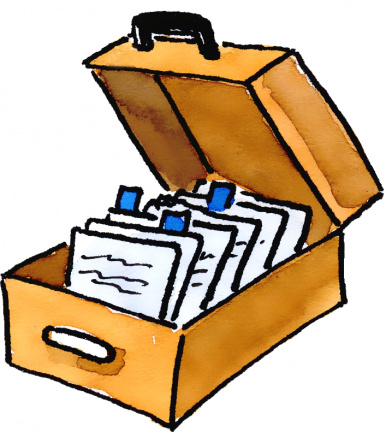
\includegraphics[width=5cm]{6.1-LT-Abb_Kartei}
		\end{wrapfigure}
		Überleg dir selber \emph{eine Lernstation} zum Thema \emph{Bruchrechnen}.
		
		Such dir zum Beispiel aus dem Buch eine Aufgabe, überlege dir mit einer Mitschülerin eine Karte oder erfinde selber eine tolle Aufgabe.
		
		Erstelle dann deine Karte auf einem Din-A5 Blatt.
		
		Deine Karte braucht auch
		\begin{smallitemize}
			\item einen Titel,
			\item eine Farbe,
			\item ein Symbol.
		\end{smallitemize}
		
		Vergiss auch nicht, auf der Rückseite \emph{die Lösung} darzustellen.

		\infotext{Bild \enquote{Datenbank} von Ute Ohlms (bidab.nibis.de)}
	\end{karte3}
	
	\leereKarte
	
\end{document}